% !TeX root = ../main.tex

\chapter{VideoABC 数据集}\label{cha:VideoABC}
VideoABC(Video ABductive Commonsense Reasoning)是专门为视频溯因推理任务而设计的一个数据集。该数据集以教程类视频数据集COIN\cite{tang2019coin}为基础进行二次标注进而构建而成。基于COIN数据集来构建VideoABC的原因主要有以下几点:
\begin{enumerate}
    \item COIN数据集是一个教程类视频的数据集,具有明确的步骤划分,每个步骤都是一个将对完整而独立的动作,适合于\VACR 的任务设定;
    \item COIN数据集中的步骤具有很强的时序关系,适合用来构建时序上的视觉推理任务;
    \item COIN数据集中的视频都来自于真实世界,从而需要模型具有对常识的理解能力;
    \item COIN 数据集是目前公开数据集中视频数目最多(11,827个),视频总时长最长(超过476h),视频种类最多(180类)。所以,以COIN为基础构建数据集,可以使得训练出来的模型适应于多种日常生活场景中的推理任务。
\end{enumerate}

本章将详细介绍 VideoABC数据集的构建方式,包括数据的二次标注,数据集的构建,以及难分样本的挖掘。最后将给出VideoABC数据集的一些例子以及统计数据。
\section{数据标注}
\subsection{标注规则}
VideoABC 数据集基于COIN数据集构建,原始的COIN数据集中已经包含了每个步骤的名称以及时间区间的标注,然而COIN的每个视频中可能会出现动作或场景的不连续。二次标注的目的就是通过标注切分点,保证切分后的每个视频的连续性。例如在一个换轮胎的视频中可能包括了多次完整的换轮胎操作,而这每一次的换轮胎操作是互相独立的,属于不同的推理过程,所以应该在相邻的两次换轮胎的操作中间标注一个切分点。再比如在冰壶比赛的视频中,包含了很多轮比赛,而这些比赛是由不同的国家代表队完成的,此时则应该在不同轮比赛之间标注切分。

为了简化表达,本节中对于步骤序列采用以下的记号:
\begin{enumerate}
    \item 用不同的字母表示不同类型的步骤。例如$A$和$B$就表示两种不同的步骤;
    \item 用多个字母相乘来表示一个步骤序列。例如$ABC$表示依次执行$A$步骤、$B$步骤和$C$步骤;
    \item 重复的动作用连乘符号$\prod$来表示。例如$\prod_{i=1}^{2}(BC)$表示步骤序列$BCBC$;
    \item 如果重复的步骤前后具有关联,则对这些步骤增加下角标。例如$\prod_{i=1}^{2}(B_iC_i)$表示步骤序列$B_1C_1B_2C_2$。这里虽然$B_1$和$B_2$属于同样的步骤,但是$B_2$的完成依赖于$B_1$的完成。
\end{enumerate}


\begin{table}[htbp]
    \caption{特殊情况的标注规则}
    \label{tab:anno_rule}
    \begin{tabu}to\textwidth{XXX[2]}\toprule
        步骤形式 & 是否切分 & 原因\\\midrule
        $A\prod_{i=1}^{n}(BC)D$ & \xmark & 整体应该看做一次任务\\
        $\prod_{i=1}^{n}(B_iC_i)$ & \xmark & 重复的动作之间具有连续性\\
        $\prod_{i=1}^{n}(BC)$ & \cmark & 重复的动作之间相互独立\\\bottomrule
    \end{tabu}
\end{table}

在实际标注中,我们发现会有一些复杂的情况,即使存在一些重复的步骤,也不应该标注切分点。经过分析之后为这些情况制定了标注规则如表~\ref{tab:anno_rule}~所示。需要注意的是,这里的重复单元为两个步骤$BC$只是为了表述方便,实际情况中可能为任意步骤的重复单元。下面对这些特殊情况进行详细的解释。
\begin{enumerate}
    \item $A\prod_{i=1}^{n}(BC)D$ 中,虽然$BC$重复了很多次,但是由于具有开始步骤$A$和结束步骤$D$,意味着从$A$到$D$才是一个完整的任务,所以不添加任何切分点;
    \item $\prod_{i=1}^{n}(B_iC_i)$ 中,重复的动作前后具有连续性。例如在贴墙纸的视频中,一面墙需要贴许多张墙纸,每一次贴墙纸是一个重复步骤,但是后一次与前一次之前存在连续性,总体上的任务应该是包含了每一次的贴墙纸。所以,这种情况下不需要标注切分点;
    \item $\prod_{i=1}^{n}(BC)$ 中,重复的动作前后不具有连续性。例如在制作工艺品的视频中,如果制作者一共制作了多个工艺品,则每个制作过程是独立的,所以应该将它们切分开来。
\end{enumerate}

以上在实际的标注过程中,还可能遇到一些其他类型的步骤形式,不过总体上把握一个原则,即保证将所有的不连续点切分开来,即可解决大部分的情况。

\subsection{标注网站}
为了加速标注,本文开发了一个标注网站,允许多名标注员同时操作。本节中将详细介绍标注网站的设计。

标注界面如图~\ref{fig:anno_tool}~所示,可以看到整个界面主要由六个部分构成:

\begin{figure}[htbp]
    \centering
    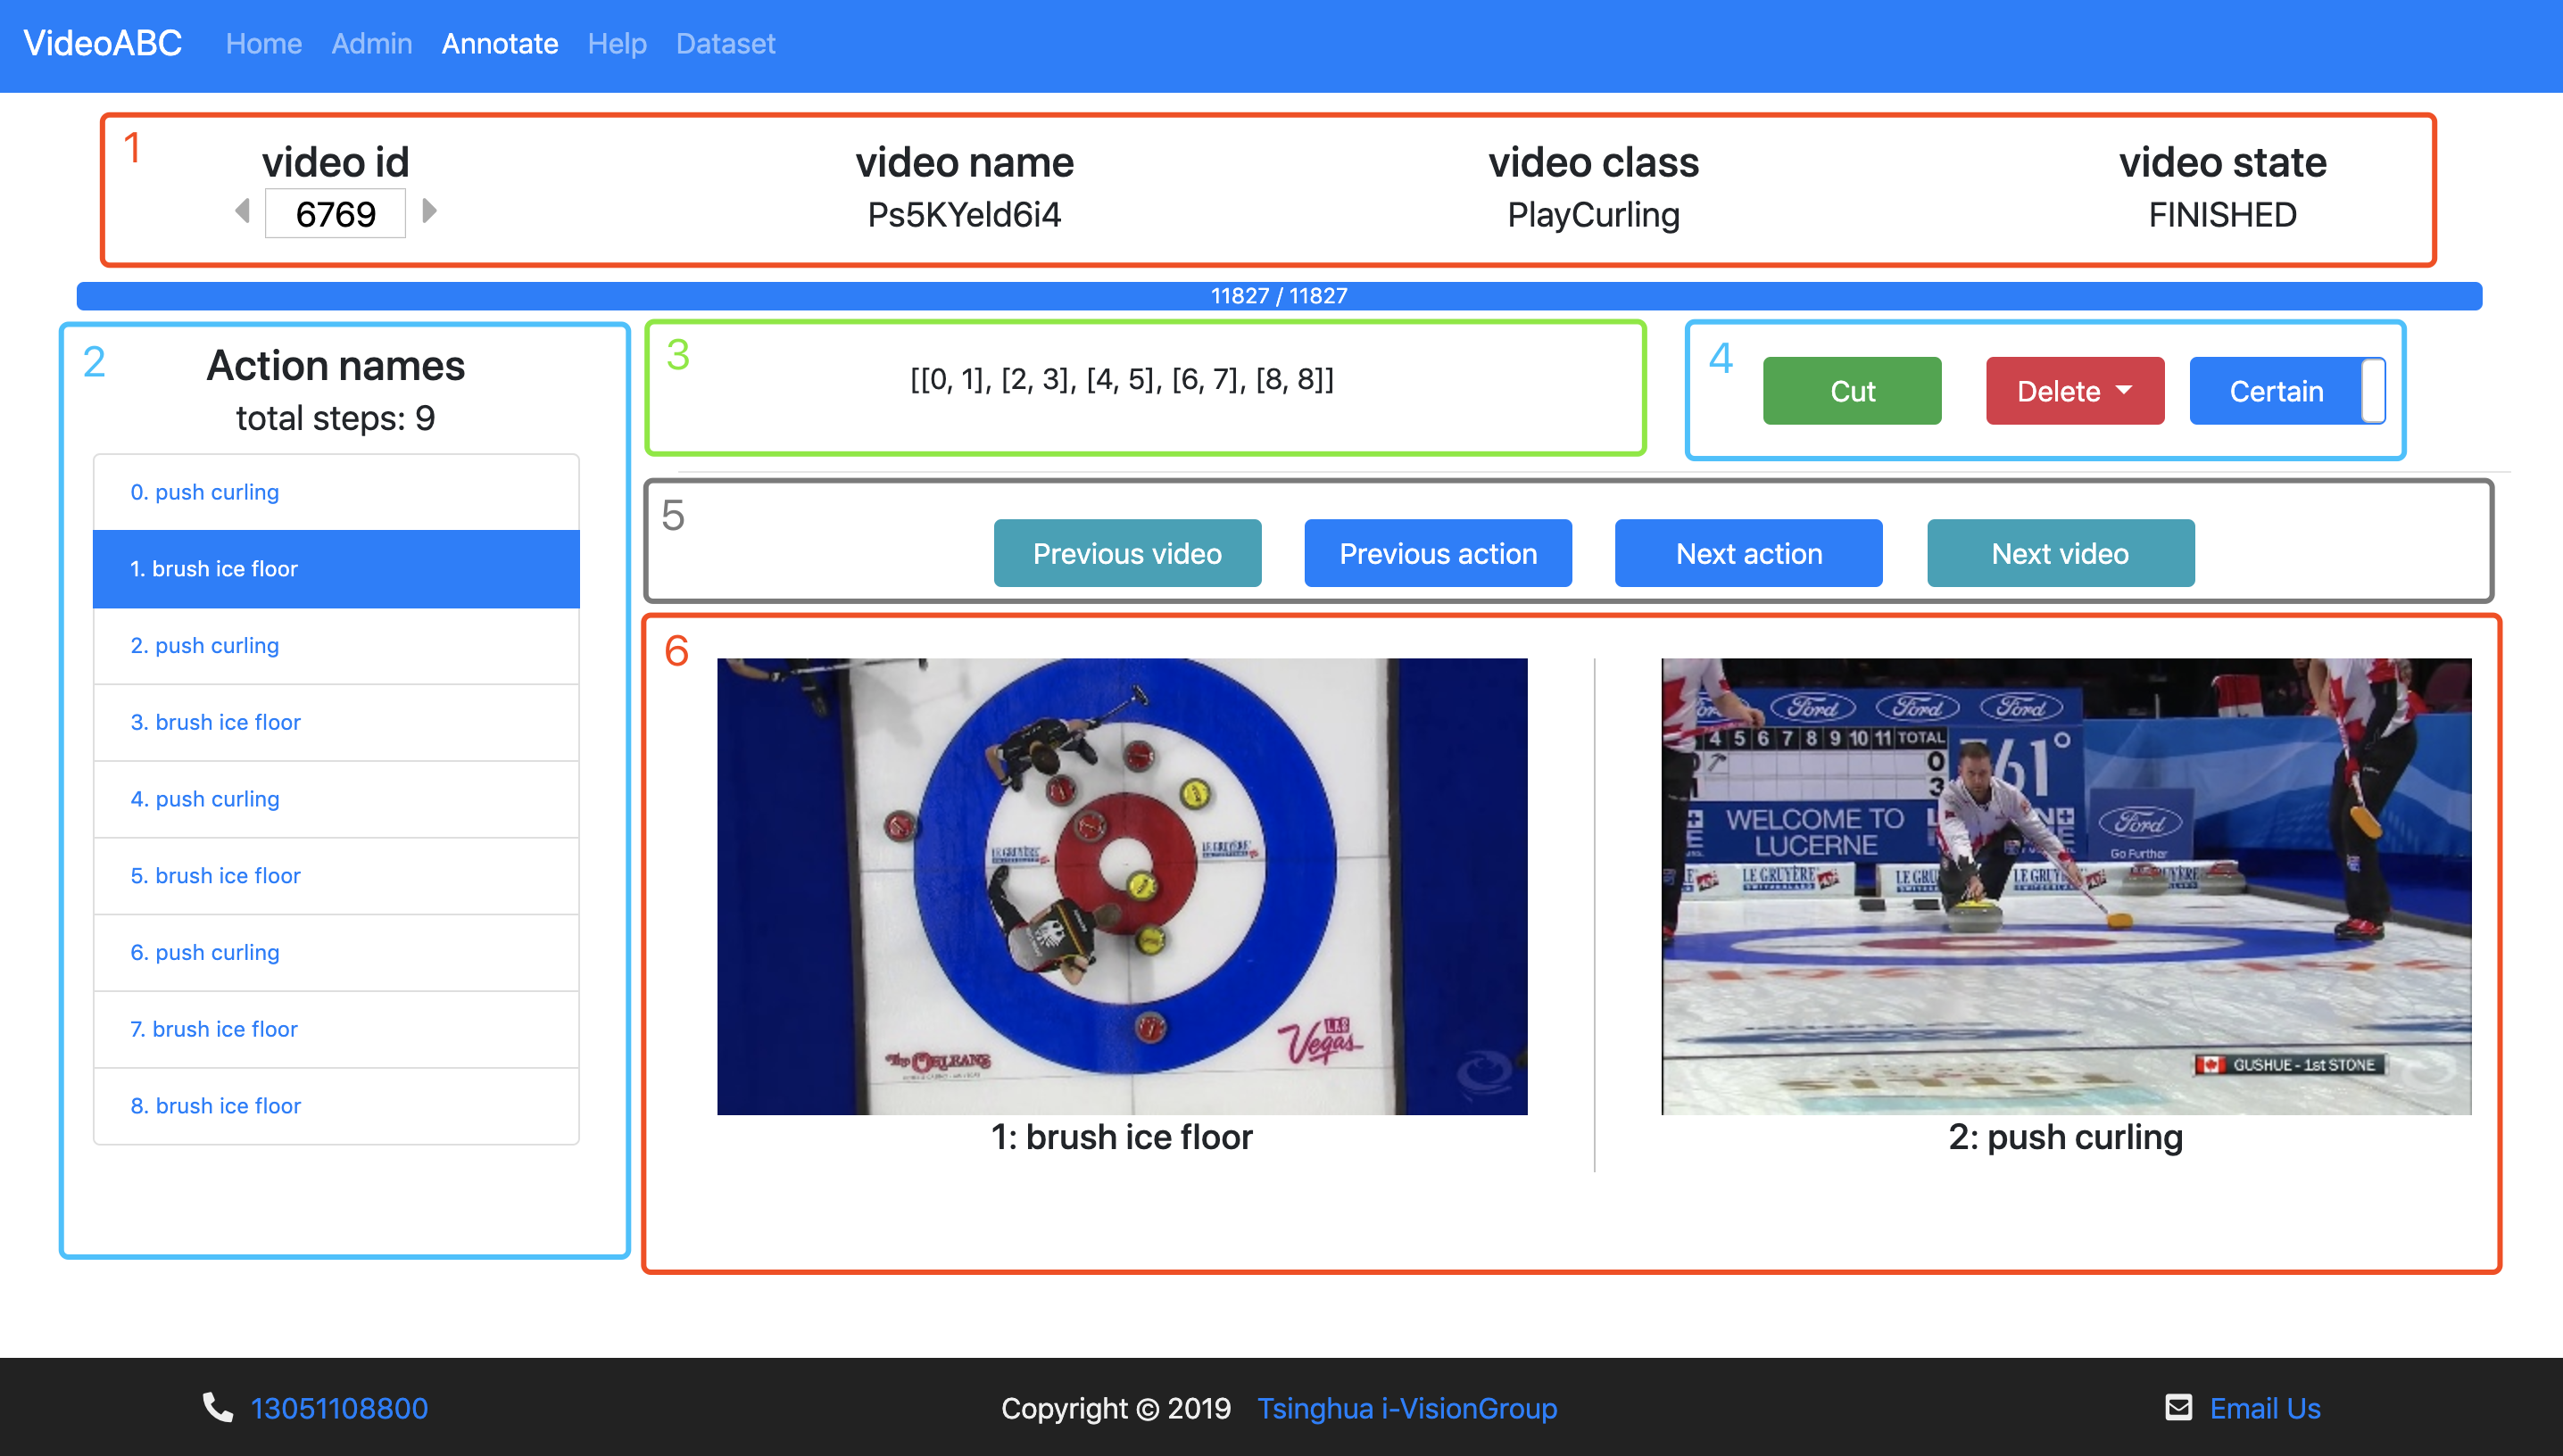
\includegraphics[width=\textwidth]{anno_tool.png}
    \caption{标注界面}
    \label{fig:anno_tool}
\end{figure}

\begin{enumerate}
    \item 基本信息区。显示了视频序号,视频名称、视频种类和视频状态。其中视频的序号是该视频在总视频中的序号,范围是1到11827(视频总数),视频名称为该视频在COIN数据集中原始的名称(来自于Youtube中的视频id),视频种类指的是该视频中的任务类型,视频状态分为三种:未标注,标注中,已标注。
    \item 动作列表区。显示了该视频中所有步骤的动作名称,以及动作总数。当前的步骤用蓝色背景标出,标注员可以点击某个步骤快速到达该步骤。
    \item 切分结果区。以列表的形式显示了当前的切分结果,该列表中的每个元素为一个闭区间,表示了每个切分后的视频区间。例如[[0, 1], [2, 3]]表示在步骤1和步骤2中间存在一个切分点。需要注意的是,这里所有的步骤序号都是从0开始计算的。
    \item 编辑区。包括三个控件:切分按钮、删除按钮、确定性开关。
    \begin{enumerate}
        \item 切分按钮:点击后会在当前步骤和下一步骤中间添加一个切分点。
        \item 删除按钮:点击后会出现一个下拉菜单,标注员可以指定删除某一个切分点或者删除所有的切分点。
        \item 确定性开关:用来表示对当前视频标注结果是否确定,默认为开启状态(确定)。一旦标注员将其切换到关闭状态(不确定)时,界面下方会出现一个文本框,可以在其中填写不确定的理由。这样我们可以在最后统一处理有疑问的视频。
    \end{enumerate}
    \item 导航区。包括四个按钮,分别为上一视频、下一视频、上一步骤、下一步骤。
    \item 关键帧区。展示了当前动作和下一动作的关键帧。由于标注的目标是找到视频中的不连续点,这里显示的是当前步骤的最后一帧和下一步骤的第一帧。如果当前步骤后存在切分点,这两张图片之间会显示一条浅灰色的竖线(如图~\ref{fig:anno_tool}~所示)。
    
\end{enumerate}


\begin{table}[!h]
    \caption{标注网站的键盘快捷键}
    \begin{tabu}to\textwidth{X[c]X[c]}\toprule
        键盘按键 & 功能\\\midrule
        \keys{A}	& 下一步骤\\
        \keys{S}	& 上一步骤\\
        \keys{F}	& 第一个步骤\\
        \keys{E}	& 最后一个步骤\\
        \keys{0}~$\sim$~\keys{9}	& 跳转到第$i$个步骤($i\in[0, 9]$)\\
        \keys{V}	& 下一视频\\
        \keys{B}	& 上一视频\\
        \keys{\arrowkeyleft}    & 上一视频 (以视频序号计算)\\
        \keys{\arrowkeyright} & 下一视频 (以视频序号计算)\\
        \keys{C}	& 切分\\
        \keys{R}	& 跳转到下一个状态为“标注中”的视频\\\bottomrule
    \end{tabu}
\end{table}

在实际标注的过程中,标注员可以先通过视频类型和左侧的动作列表中来了解该视频中任务的特点。对于每个视频,标注员在多个情况下都可以直接通过动作列表中的文本来找到重复的步骤单元,从而能够快速定位切分点并标注。另外,为了加速标注,一些常用的操作都绑定了键盘快捷键,包括步骤和视频的跳转、切分点的编辑等等。需要注意的是,这里的快捷键“V”表示的“下一视频”指的是下一个未标注的视频。如果想跳转到按照视频序号的下一视频应该按向右方向键。

为了统一标注的标准,标注网站的导航栏中设置了“Help”标签页,用来显示帮助信息,其中包括了标注规则、标注方法和标注快捷键,如图~\ref{fig:help}~所示。

\begin{figure}[htbp]
    \centering
    
\includegraphics[width=\textwidth]{help.png}
    \caption{标注网站的帮助页面}
    \label{fig:help}
\end{figure}

\subsection{标注网站的实现细节}
本节将详细介绍标注网站的实现细节。
\subsubsection{后端}
标注网站的后端基于Django\cite{django}框架构建。一个Django工程中可以包含多个应用(app),例如本节中介绍的标注工具就是一个应用,我们将其命名为anno(annotation)。anno 文件夹下的目录如下(仅列出主要的文件和目录):
\begin{enumerate}
    \item anno/
    \begin{enumerate}
        \item models.py
        \item views.py
        \item urls.py
        \item static/
        \item templates/
        \item ...
    \end{enumerate}
\end{enumerate}
其中,models.py 中定义了数据结构,urls.py 中定义了各个网页的url,views.py 中定义了每个网页的传入内容和跳转关系,templates 目录中的 HTML 模板用来渲染每个网页,static 目录中用来存放一些固定不变的文件(如图片、视频、CSS 等等)。下面介绍后端的一些重要组成部分,包括数据结构、URL定义和页面跳转逻辑,以及它们的实现方式。

\paragraph{数据结构} 首先需要定义数据结构,即标注结果的存储方式。由于我们的标注是以视频为单位进行的,这里的数据结构也应该以视频为单位。具体来说,我们定义Video类如表~\ref{tab:video_vars}~所示。大部分的内容在表中已经表达得很清楚,但仍有一些需要明确:
\begin{enumerate}
    \item action\_ids 是指该视频中的动作在COIN数据集中\emph{所有}动作的序号,不同的动作用逗号分隔开。
    \item cut\_points 中不同的切分点用逗号分隔,例如“1,2,5”表示在步骤1、步骤2、步骤5后添加切分点。
    \item note 只在 certainty 被置为False时才可写入。
    \item prev\_vid 是指当前编辑视频之前所编辑的视频的序号。
\end{enumerate}

Video类定义在models.py中,Django框架可以自动为其链接到数据库(本文使用SQLite数据库),所有的Video对象被保存在数据库中的一张表中,数据域与成员变量相对应。
\begin{table}
    \caption{Video类成员变量}
    \label{tab:video_vars}
    \begin{tabu}to\textwidth{XXX}\toprule
        变量名称 & 变量类型 & 变量含义\\\midrule
        video\_name & 字符串 & 视频名称\\
        video\_class  & 字符串 & 视频类型\\
        steps & 小正整型 & 步骤总数\\
        action\_ids & 字符串 & 动作序号\\\midrule
        cut\_points & 字符串 & 切分点\\
        state & 小正整型 & 视频状态\\
        certainty & 布尔型 & 确定性\\
        note & 字符串 & 备注\\
        prev\_vid & 小正整型 & 上次编辑的视频序号\\
        checkpoint & 小正整型 & 上次编辑的步骤序号\\\bottomrule
    \end{tabu}
\end{table}

\paragraph{URL 定义} 表~\ref{tab:urls}~中给出了 anno 中用到的主要URL定义、绑定的函数以及对应的含义。Django使用URL模式(URL patterns)的方法来定义一个通用的格式(相对路径),并对这个URL模式绑定一个函数(在views.py中定义),具体访问URL的时候再将URL中的参数传入到函数里可进行处理。例如,如果app部署的根路径为“localhost:8888/anno”,则访问链接“localhost:8888/anno/1/0” 时内部的实现逻辑如下:
\begin{enumerate}
    \item Django按照格式和变量类型从anno中所有预定义的URL模式中匹配“1/0”,发现只有 “<int:video\_id>/<int:start\_step>”符合。
    \item 通过该URL模式,找到了绑定的函数views.anno函数。
    \item 将“video\_id=1, start\_step=0”作为参数传入views.anno函数调用。
    \item views.anno 函数中通过访问数据库得到需要显示的内容,并传给HTML模板渲染。
\end{enumerate}

可以看到,表~\ref{tab:urls}~中除了标注界面,其他的URL模式都属于用来过渡的URL。这些URL模式的设置是为了方便通过调用函数的形式与数据库交互,最终都会回到标注界面。

\begin{table}
    \caption{URL模式的定义}
    \label{tab:urls}
    \begin{tabu}to\textwidth{X[1.5]XX}\toprule
        URL 模式 & 绑定函数 &含义\\\midrule
        <int:video\_id>/<int:start\_step> & views.anno & 标注界面\\ 
        start/ & views.start &开始(过渡)\\
        resume/& views.resume &恢复(过渡)\\
        <int:video\_id>/navigate & views.navigate &导航(过渡)\\
        <int:video\_id>/edit & views.edit &编辑(过渡)\\\bottomrule
    \end{tabu}
\end{table}
\paragraph{页面跳转逻辑} 表~\ref{tab:urls}~中已经给出了URL模式的定义,下面介绍它们之间的页面跳转逻辑。
\begin{enumerate}
    \item 访问标注界面时,后端会调用 views.anno 函数,根据video\_id 从数据库中读取对应视频条目,根据start\_step 选定当前步骤,将所有需要显示的信息(视频基本信息、关键帧路径、标注进度等)传入HTML模板中渲染。
    \item 点击动作列表区的步骤,会改变当前的步骤序号并重新加载标注页面。
    \item 按下导航区的某个按钮时会发送表单到 <int:video\_id>/navigate ,进而调用views.navigate 函数。在函数内部通过读取表单信息,确定导航后的视频序号、步骤序号,再重定向到标注页面。
    \item 按下编辑区的按钮时会发送表单到<int:video\_id>/edit,并调用views.edit 函数。函数内部会读取表单信息,决定执行添加切分点、删除切分点或者改变确定性的操作。编辑结束后再重定向回标注页面。
   \item 执行步骤之间的导航操作时,views.navigate 函数会将当前的步骤记录在checkpoint中,便于记录进度。
   \item 点击下一视频按钮时,将当前视频状态更改为标注完成,并选择一个未标注的视频作为下一视频,将下一视频的“prev\_id”变量更改为当前视频的序号。
   \item 按下快捷键“R”时,跳转到resume/ 并调用 views.resume 函数,寻找数据库中处于“标注中”状态的视频并跳转到该视频的标注界面。
   \item 在标注网站的主页(图~\ref{fig:anno_index}~)中有两个按钮,分别为继续上一标注(Continue)和开始新标注(Start new)。若选择继续上一标注,则跳转到resume/页面;若选择开始新标注,则跳转到start/页面,通过调用views.start 函数,在数据库中选择一个未标注过的视频并跳转到该视频的标注页面。
\end{enumerate}

以上的这些跳转逻辑在实现标注功能的同时保证了线程安全,确保可以多个标注员同时标注而不发生冲突。其中视频状态的设计相当于加锁,保证一位标注员在对某个视频标注的过程中其他标注员不会访问到同样的视频。

\begin{figure}[htbp]
    \centering
    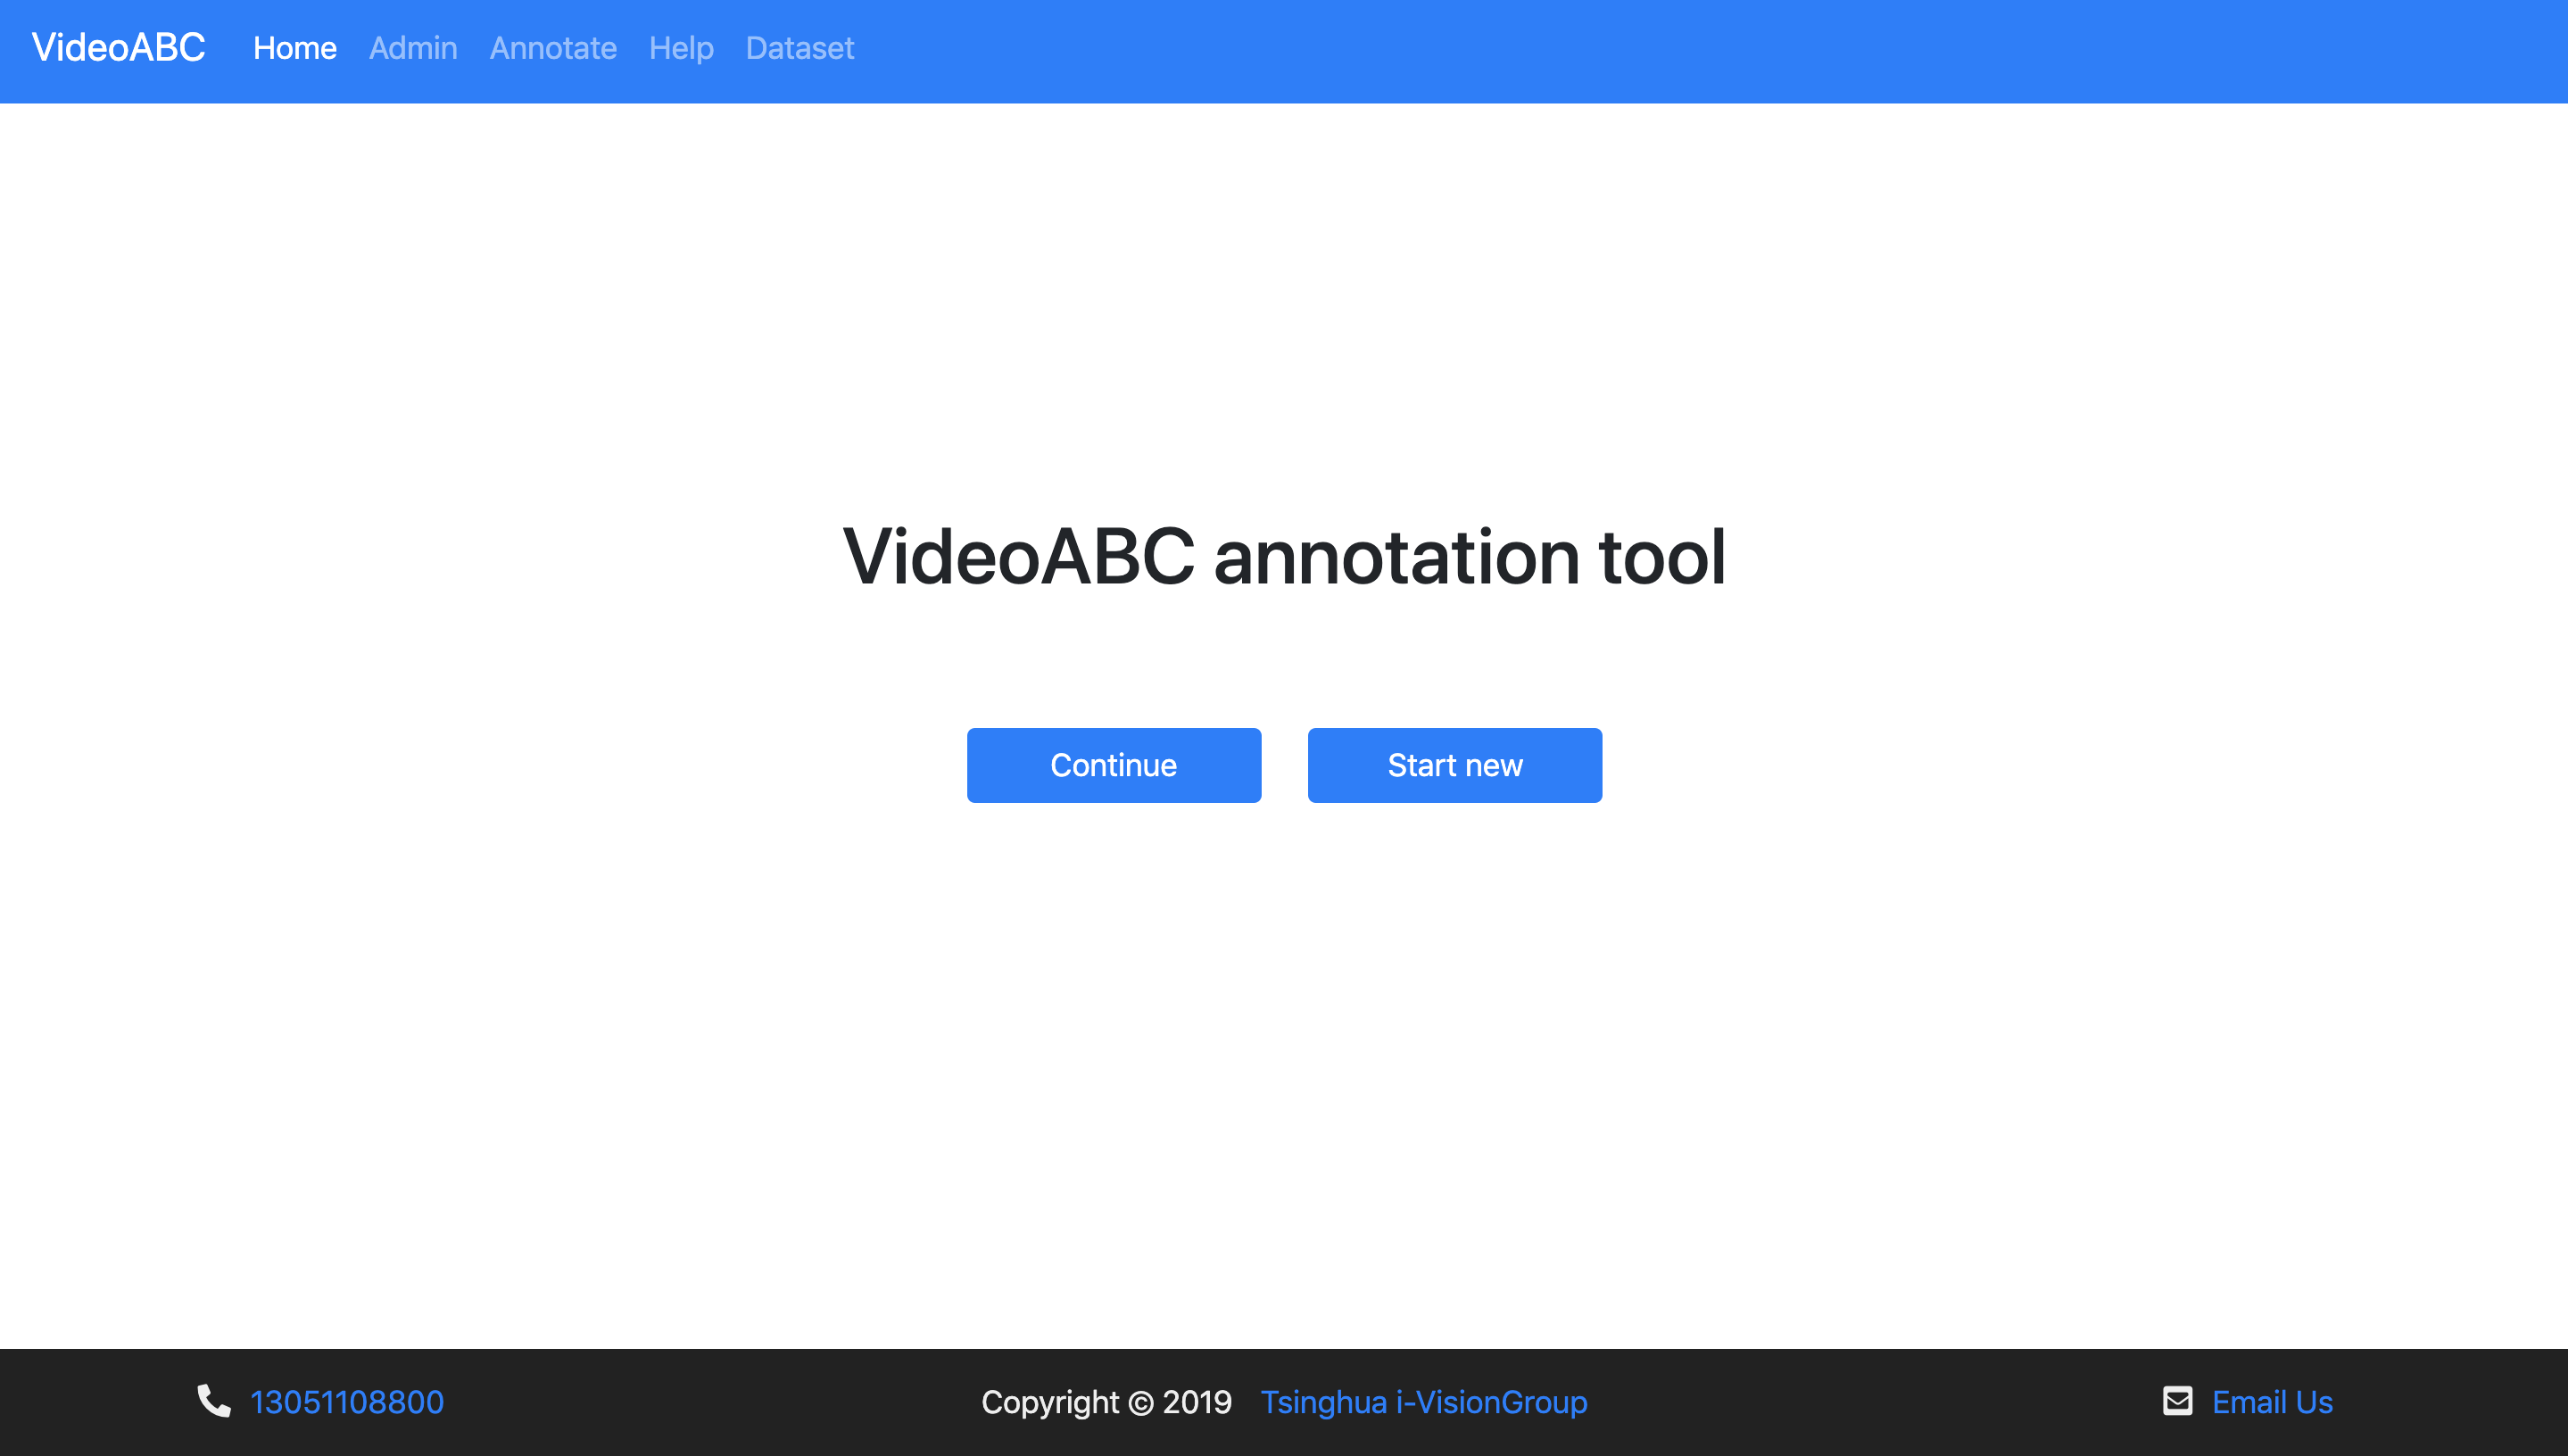
\includegraphics[width=\textwidth]{index.png}
    \caption{标注网站主页}
    \label{fig:anno_index}
\end{figure}
\subsubsection{前端}
标注网站的前端使用HTML+CSS+JavaScript 构建。其中HTML负责基本排版,CSS负责样式渲染,JavaScript用来实现各种快捷键操作。为了统一风格,本文使用了Bootstrap\cite{bootstrap}库完成了大部分的排版和渲染。使用Bootstrap 有以下几个好处:
\begin{enumerate}
    \item 包括了大量的预定义样式,例如按钮、导航栏、表单等等,可节省大量的CSS代码编写量。且风格统一,简洁而不失美观。
    \item 调用十分方便,只需在代码中添加几行就可以使用。
    \item 复用性强,目前很多网站中都在使用Bootstrap框架,所以大部分的浏览器中都已经预先下载过Bootstrap中的资源,避免了资源文件的重复下载。
    \item 具有多种使用的便于使用的布局工具,例如流动性容器可以使控件根据屏幕大小自动调整,便于从不同的客户端访问标注网站。
\end{enumerate}

\section{数据集构建}
\subsection{视频切分与筛选}
\label{sec:filter}
在标注数据的过程中,我们已经在视频中的不连续位置标记了切分点,但是即使这样,切分后的视频中的步骤数目仍然相差很大。为了便于处理,我们需要设置步骤数目的限制。另外,我们还需要保证训练集和测试集中的视频片段分布的均匀性。设原始的视频数据集为$\gD=\{D_i\}$,则视频切分与筛选的算法如下:
\begin{enumerate}
    \item 使用标注的切分点将视频切分,得到数据集$\gD'$;
    \item 给定最小步骤数$m=2$和最大步骤数$M=6$;
    \item 利用$m$和$M$对$\{D_i'\}$进一步处理,即对步骤数大于$M$的进行再次切分,对步骤数少于$m$的直接去除,得到数据集$\gD''$;

\end{enumerate}
经过上述算法后,我们已经得到了清洗后的数据集$\gD''$,其中每个样本中的步骤数目都在$m$到$M$之间。基于$\gD''$的每个样本,可以按照如下步骤来构建正确选项:
\begin{enumerate}
    \item 对每个步骤按照COIN的原始标注的时间区间抽取16帧;
    \item 第一个步骤的第一帧作为$O_1$,最后一个步骤的最后一帧作为$O_2$;
    \item 截取每个步骤的\emph{中间}8帧作为最终使用的视频片段,构成正确假设$H_+$。
\end{enumerate}

上述的做法保证了两个观测$O_1$和$O_2$不会直接出现在$H_+$的帧中。否则如果$H_+$里直接使用16帧,或等间隔抽8帧都会出现这种情况,导致模型只需要做简单的比对就能得出答案。

接下来对数据集进行划分。定义训练集比例$\alpha$,划分训练集和测试集,保证:
\begin{enumerate}
    \item $\gD''$中来自于同一个原始视频的必须同时被划分到训练集或测试集;
    \item 同一类别的视频中,训练样本的比例尽可能接近$\alpha$。
\end{enumerate}
至此,我们已经得到了训练集和测试集的所有观测和正确假设。
\subsection{错误假设生成}
本节介绍如何根据正确假设来生成错误的假设集合$\gH_-$。VideoABC数据集中共包括四种错误类型:
\begin{enumerate}
    \item 删除(remove)一个步骤;
    \item 交换(swap)两个步骤;
    \item 插入(insert)一个步骤;
    \item 替换(replace)一个步骤。
\end{enumerate}
正是因为有这几种错误类型,我们在之前对视频切分和筛选时才指定了一个最小步骤数$m=2$,否则swap和remove两种错误类型将不存在,insert则可以通过判断步骤数简单排除,只剩下replace 的错误类型可供选择。对于每个问题,我们会均匀生成各种错误类型的选项,从中选取三个,与正确选项一起,构成一个四选一的选择题。
\subsection{难分选项挖掘}
构建VideoABC时的一个关键的地方在于能够生成出高质量的干扰选项,从而使得任务更有挑战,更能筛选出推理能力强的模型。为了去除过于明显的错误假设,本文使用了难分选项挖掘(Hard Choice Mining)的方法来提高难度。具体步骤如下:
\begin{enumerate}
    \item 使用上一节的方法生成错误选项得到初始的数据集;
    \item 在初始的数据集上训练一些基础模型,并选出表现最好的;
    \item 对每个样本再次生成错误选项,每种类型错误选项生成不超过15个,利用预训练模型选出其中分数最高的3个,构成新的数据集;
\end{enumerate}
通过不断重复上述步骤,最终得到的数据集中的错误选项都是具有一定的干扰性的,从而提高了VideoABC数据集的难度。

\section{VideoABC数据集}
在本章前面几节中,我们已经详细地介绍了VideoABC数据集的构建方式,下面介绍VideoABC中的一些统计数据。
\begin{figure}[htbp]
    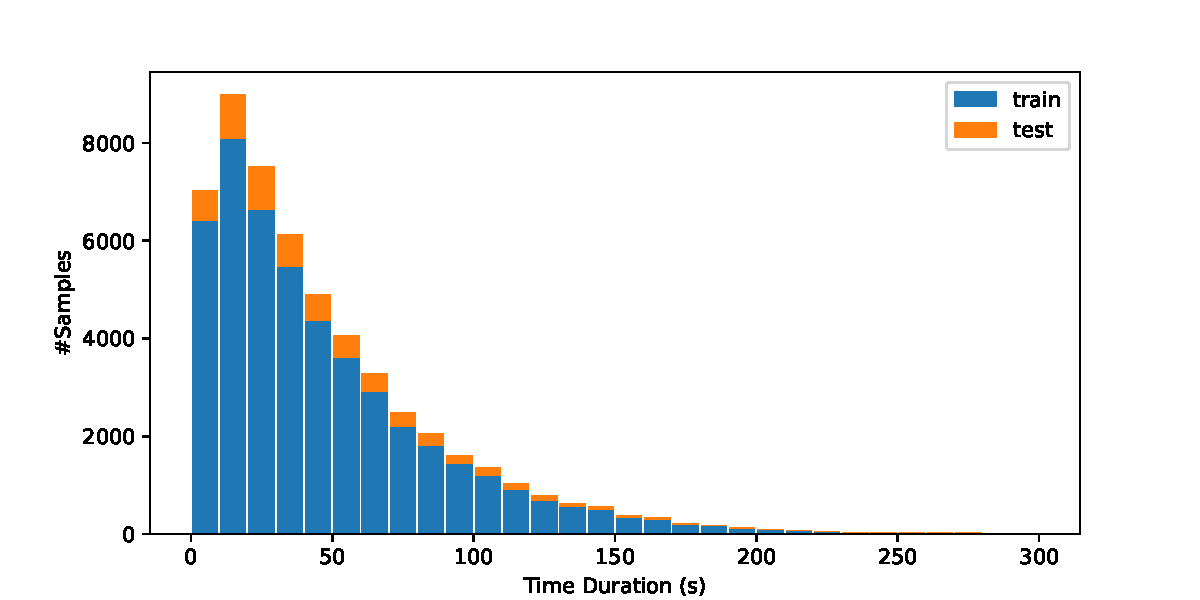
\includegraphics[width=\textwidth]{duration.pdf}
    \caption{VideoABC 的推理时长分布}
    \label{fig:duration}
\end{figure}

图~\ref{fig:duration}~中展示了VideoABC中的推理时长的分布(仅展示0$\sim$300s之间),横坐标为推理时长,纵坐标为选项个数。可以看到VideoABC中的推理时长是一个长尾分布,主要分布在0$\sim$200s之间。可见模型要想在该数据集上取得良好的表现,必须具有能够对长期和短期视觉信息推理的能力。

\begin{figure}[htbp]
    \centering
    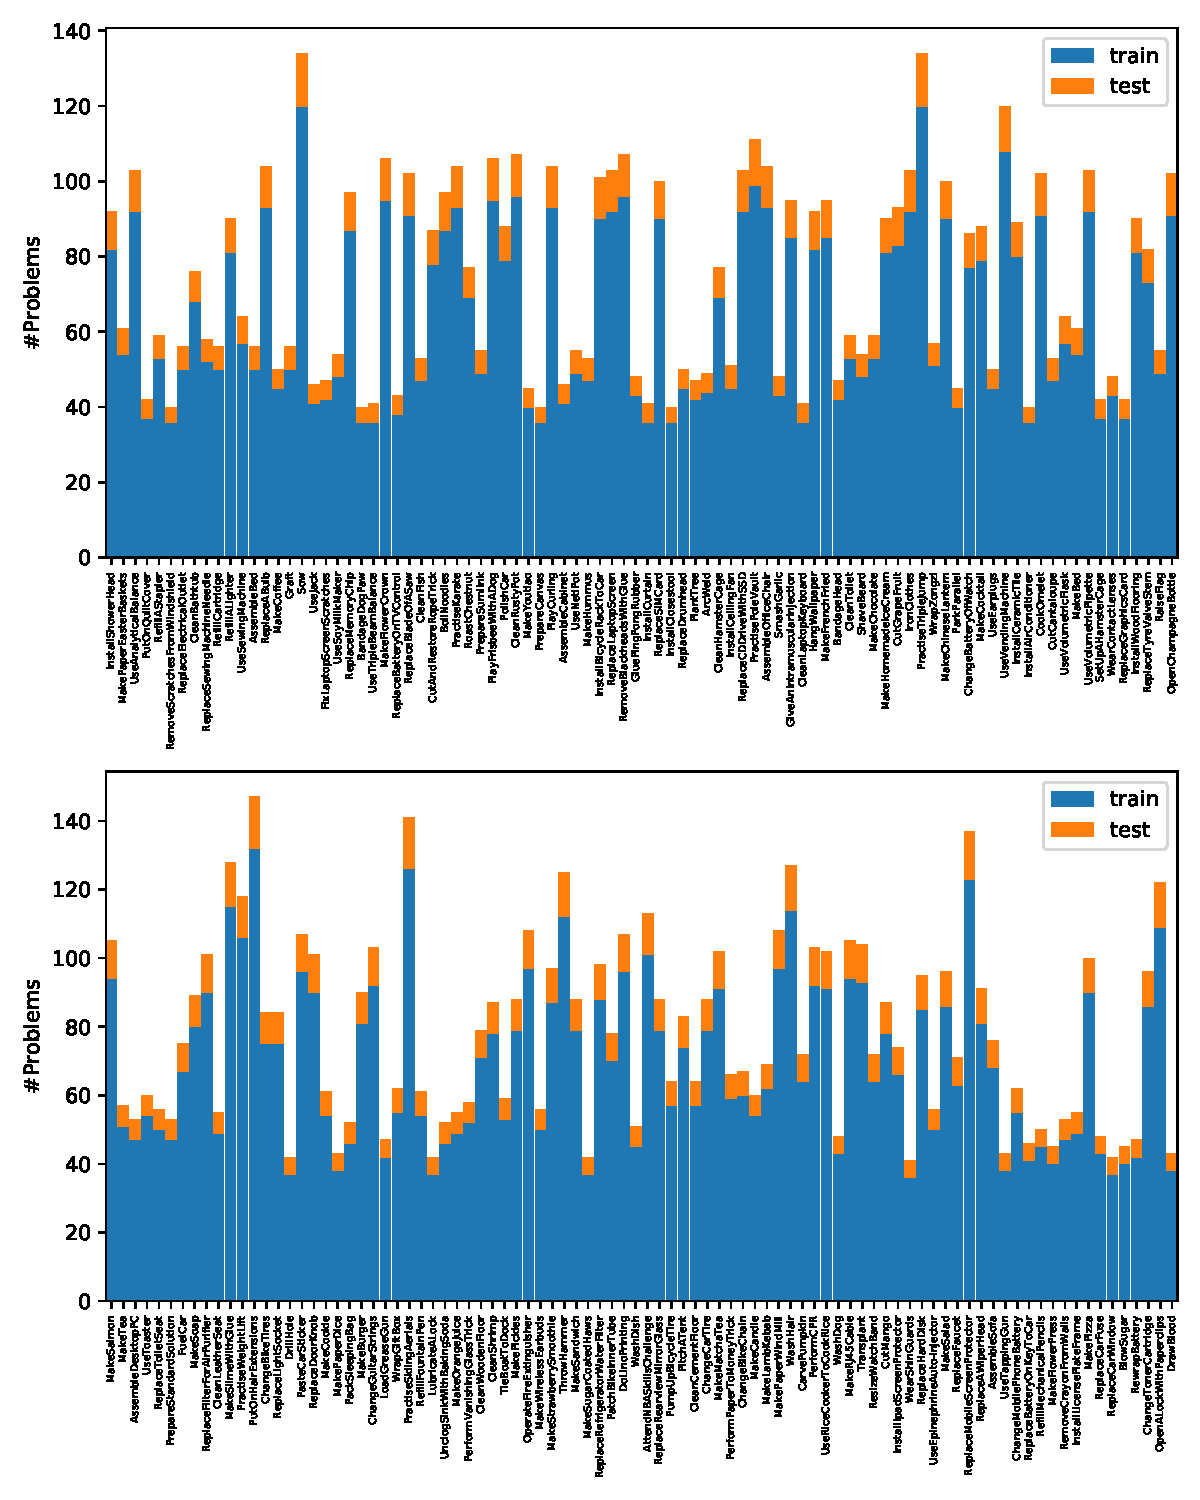
\includegraphics[width=\textwidth]{tasks.pdf}
    \caption{VideoABC 中任务分布}
    \label{fig:tasks}
\end{figure}
图~\ref{fig:tasks}~中展示了VideoABC总的任务种类分布,其中横轴为任务种类,纵轴为对应的问题数。VideoABC中包含180中任务种类(与COIN数据集中的任务种类一致),涵盖生活中的各种场景
从图中可以看出,每种任务种类中训练集的比例均接近90\%。

\begin{figure}[htbp]
    \centering
    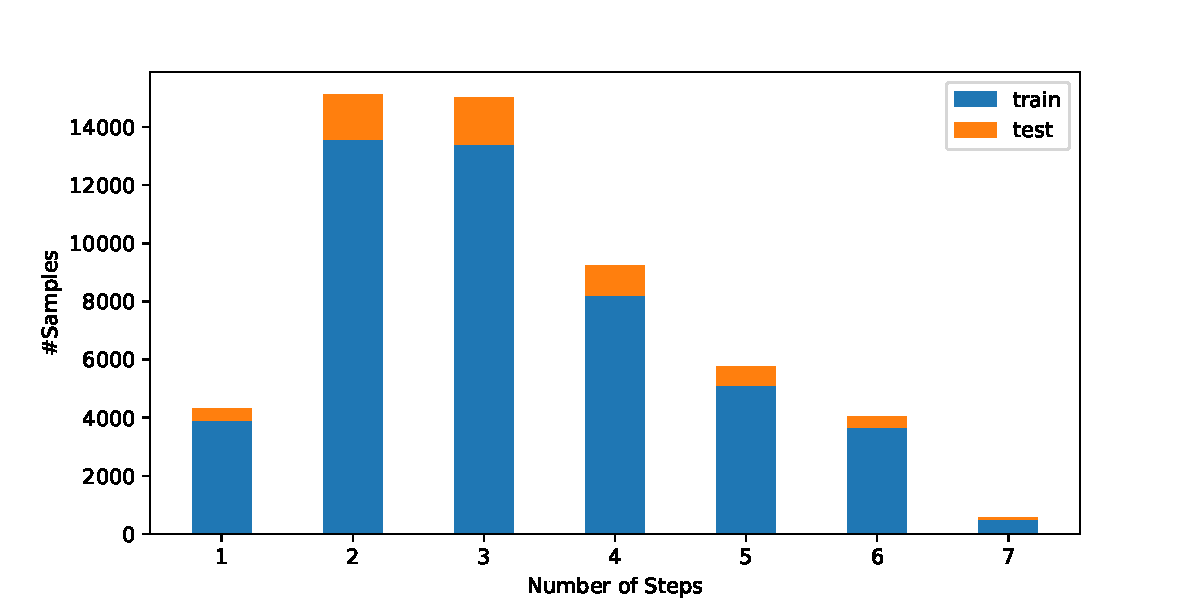
\includegraphics[width=\textwidth{}]{steps.pdf}
    \caption{VideoABC 选项中步骤数分布}
    \label{fig:steps}
\end{figure}

图~\ref{fig:steps}~展示了VideoABC中的步骤数的分布。在第~\ref{sec:filter}~里,我们曾指定了\emph{正确}选项的最小步骤数$m=2$和最大步骤数$M=6$。再将四种错误类型考虑进去,可知\emph{所有}选项的最大步骤数是$M+1=7$(正确选项步骤数为6,错误类型为插入),最小步骤数是$m-1=1$(正确选项步骤数为2,错误类型为删除)。所以可以看到,VideoABC中的步骤数分布在1$\sim$7之间,但是步骤数是1或7的选项都比较少。

\begin{figure}[htbp]
    \centering
    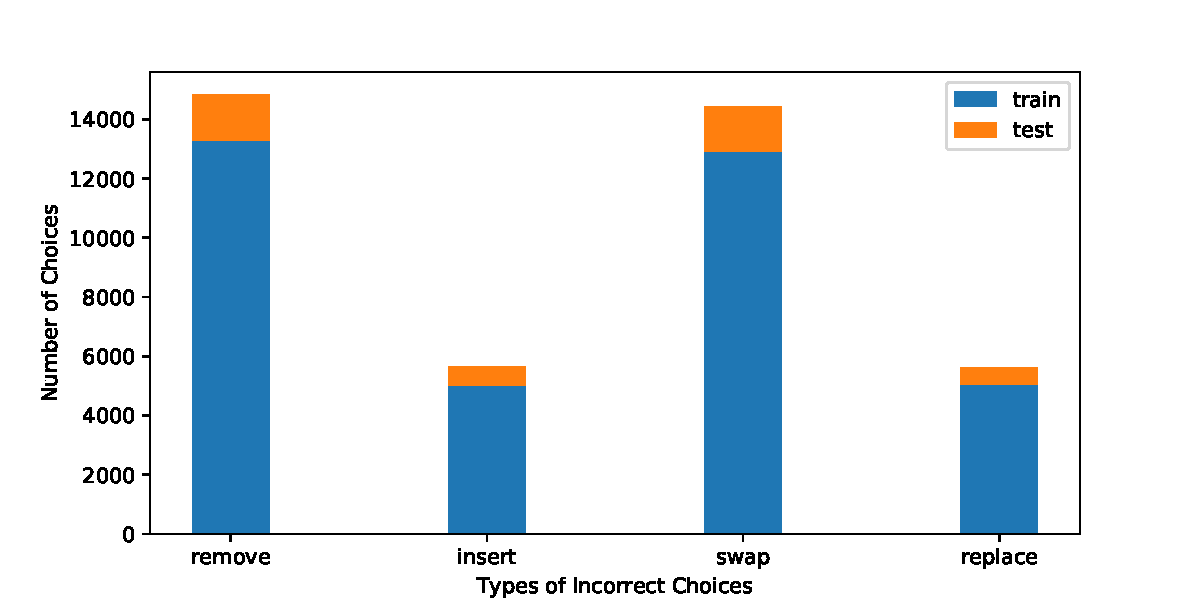
\includegraphics[width=\textwidth]{types.pdf}
    \caption{VideoABC 选项中错误类型的分布}
    \label{fig:wrong_types}
\end{figure}

图~\ref{fig:wrong_types}~中展示了VideoABC选项中错误类型的分布。可以看到,四种类型的错误选项并不是均匀分布,这就体现了难分选项挖掘的作用。经过难分样本挖掘之后,留下来的错误选项都是一些比较具有干扰性的。由此可以看出,删除和交换两种错误类型是比较困难的,而插入和替换两种错误类型是比较简单的。

\begin{table}[htbp]
    \caption{VideoABC的统计数据}
    \label{tab:stat}
    \begin{tabu}to\textwidth{XX}\toprule
        名称 & 统计数据\\\midrule
        原始视频数 & 11,827\\
        任务种类数 & 180\\
        步骤类型数 & 778\\\midrule
        步骤总数 & 46,354\\
        问题总数 & 13,522\\
        训练集问题总数 & 12,086\\
        测试集问题总数 & 1,436\\\midrule
        最大推理时长 & 731s\\
        平均推理时长 & 47s\\\bottomrule
    \end{tabu}
\end{table}

表~\ref{tab:stat}~中展示了VideoABC数据集的一些统计数据。由于VideoABC数据集是基于COIN数据集构建的,VideoABC具有多种多样的任务种类和步骤类型。VideoABC中共有13,522个问题,其中训练集中有12,086个,测试集中有1,436个。另外可以看到,VideoABC中推理时长的范围非常大,最大可达731s,平均推理时长为47s,模型必须能够适应长时间的推理任务才能在VideoABC上取得良好的表现。

\begin{figure}[]
    \begin{subfigure}{\textwidth}
        \centering
        \includegraphics[width=.8\textwidth,page=1]{VideoABC.pdf}
        \caption{}
    \end{subfigure}
    \begin{subfigure}{\textwidth}
        \centering
        \includegraphics[width=.8\textwidth,page=2]{VideoABC.pdf}
        \caption{}
    \end{subfigure}
    \begin{subfigure}{\textwidth}
        \centering
        \includegraphics[width=.8\textwidth,page=3]{VideoABC.pdf}
        \caption{}
    \end{subfigure}
    \begin{subfigure}{\textwidth}
        \centering
        \includegraphics[width=.8\textwidth,page=4]{VideoABC.pdf}
        \caption{}
    \end{subfigure}
    \caption{VideoABC数据集示例}
    \label{fig:illu}
\end{figure}
图~\ref{fig:illu}~展示了VideoABC数据集中的一些例子。在VideoABC数据集中,每个问题中都有一个正确选项和三个错误选项,图~\ref{fig:illu}~中则对每个问题只展示了一个正确选项一个错误选项。其中错误选项的错误类型已经用文字和虚线框标出。在实际的数据集中,每个选项中的步骤其实是一个视频片段,而图中只显示了视频片段的最中间的一帧。图~\ref{fig:illu}~中的四个子图分别对应着四种错误类型:插入、删除、交换、替换。同时,图~\ref{fig:illu}~中的例子属于不同类型的任务(烹饪、小制作、修理、体育运动),由此也可以看出VideoABC数据集中推理场景的多样性。

实验发现,一些最先进的的视频理解模型在VideoABC上都没能取得很好的表现,(具体的实验结果会在第~\ref{cha:experimetns}~章介绍)。为了解决这个问题,我们有必要针对视频溯因推理的特点来重新设计模型结构。